% !TEX program = xelatex
\documentclass[12pt,a4paper]{report}

% ── Fonts ────────────────────────────────────────────────────────────────────
\usepackage{fontspec}
% Template fonts are Times New Roman / Arial; fall back to metric-compatible
% Liberation, then to TeX Gyre (bundled with TeX Live) where unavailable.
\IfFontExistsTF{Times New Roman}{\setmainfont{Times New Roman}}{%
  \IfFontExistsTF{Liberation Serif}{\setmainfont{Liberation Serif}}%
    {\setmainfont{TeX Gyre Termes}}}
\IfFontExistsTF{Arial}{\setsansfont{Arial}}{%
  \IfFontExistsTF{Liberation Sans}{\setsansfont{Liberation Sans}}%
    {\setsansfont{TeX Gyre Heros}}}

% ── Page geometry ─────────────────────────────────────────────────────────────
% Left 4 cm, others 2 cm  (Oulu IPS template)
\usepackage[
  a4paper,
  left=4cm,
  right=2cm,
  top=2cm,
  bottom=2cm,
  includeheadfoot,
  headheight=15pt
]{geometry}

% ── Line spacing ──────────────────────────────────────────────────────────────
\usepackage{setspace}
\singlespacing

% ── Headers / footers ─────────────────────────────────────────────────────────
\usepackage{fancyhdr}
\pagestyle{fancy}
\fancyhf{}
\fancyhead[R]{\thepage}
\renewcommand{\headrulewidth}{0pt}
% Chapter opening pages use the "plain" style; give it the same top-right number.
\fancypagestyle{plain}{%
  \fancyhf{}%
  \fancyhead[R]{\thepage}%
  \renewcommand{\headrulewidth}{0pt}%
}

% ── Chapter / section heading fonts  ─────────────────────────────────────────
\usepackage{titlesec}

% Chapter heading: Arial 18pt bold, no "Chapter N" prefix
\titleformat{\chapter}[block]
  {\sffamily\fontsize{18}{22}\bfseries}
  {\thechapter.}{0.5em}{}
\titlespacing*{\chapter}{0pt}{0pt}{12pt}

% Section heading: Arial 14pt bold
\titleformat{\section}[block]
  {\sffamily\fontsize{14}{18}\bfseries}
  {\thesection}{0.5em}{}
\titlespacing*{\section}{0pt}{18pt}{6pt}

% Subsection heading: Arial 14pt (not bold, matching template)
\titleformat{\subsection}[block]
  {\sffamily\fontsize{14}{18}\normalfont}
  {\thesubsection}{0.5em}{}
\titlespacing*{\subsection}{0pt}{12pt}{4pt}

% Unnumbered chapter (Abstract, Foreword, etc.) — same style, no number
\newcommand{\unnumberedchapter}[1]{%
  \chapter*{#1}%
  \addcontentsline{toc}{chapter}{#1}%
}

% ── Paragraph spacing ─────────────────────────────────────────────────────────
\setlength{\parindent}{0pt}
\setlength{\parskip}{10pt}

% ── Text alignment ────────────────────────────────────────────────────────────
\usepackage{ragged2e}
\justifying
% No words split across lines: no hyphenation, and no line breaks at explicit
% hyphens or em dashes (---). The extra inter-word stretch below lets justified
% lines absorb the words that can no longer be split.
\hyphenpenalty=10000
\exhyphenpenalty=10000
\setlength{\emergencystretch}{3em}

% ── Tables ────────────────────────────────────────────────────────────────────
\usepackage{booktabs}
\usepackage{tabularx}
% Table text is left-aligned: justified narrow cells stretch badly without hyphenation.
\renewcommand{\tabularxcolumn}[1]{>{\raggedright\arraybackslash}p{#1}}
\usepackage{array}
\usepackage{longtable}
% Figures and tables never float past the start of the next section.
\usepackage[section]{placeins}
% Pages holding only figures/tables start at the top instead of centring them.
\makeatletter
\setlength{\@fptop}{0pt}
\setlength{\@fpsep}{12pt}
\makeatother
\usepackage{makecell}

% Table caption: Arial 10pt bold, above table
\usepackage{caption}
\captionsetup[table]{
  font={sf,small,bf},
  labelsep=space,
  justification=raggedright,
  singlelinecheck=false,
  position=above
}
\captionsetup[figure]{
  font={sf,small,bf},
  labelsep=period,
  justification=centering,
  position=below
}

% ── Graphics ──────────────────────────────────────────────────────────────────
\usepackage{graphicx}
\usepackage{tikz}
\usetikzlibrary{positioning, arrows.meta, fit, calc, shapes.geometric}

% ── Hyperlinks ────────────────────────────────────────────────────────────────
\usepackage[hidelinks]{hyperref}
\usepackage{xurl}                    % allow long URLs/DOIs to break across lines

% ── Math ─────────────────────────────────────────────────────────────────────
\usepackage{amsmath}
\usepackage{amssymb}

% ── Misc ──────────────────────────────────────────────────────────────────────
\usepackage{enumitem}
\usepackage{microtype}
\usepackage{eurosym}
\usepackage{xcolor}

% ── Hanging references ────────────────────────────────────────────────────────
\usepackage{hanging}

% ══════════════════════════════════════════════════════════════════════════════
\begin{document}

% ── COVER PAGE ──────────────────────────────────────────────────────────────
% Cover follows Thesis_template_2021.docx: own 2 cm margins on all sides,
% logo centred 3 cm below the top margin, title 3.53 cm below the logo,
% author block at the page bottom indented 10.16 cm.
\newgeometry{left=2cm, right=2cm, top=2cm, bottom=2cm, nohead, nofoot}
\begin{titlepage}
\setlength{\parskip}{0pt}
\centering
\vspace*{3cm}

\includegraphics[width=3.76cm, keepaspectratio]{attachments/uni_logo.jpeg}\par
\vspace{3.53cm}
{\sffamily\fontsize{20}{24}\bfseries
A Hierarchical ReAct Multi-Agent Pipeline for Residential Appliance Load
Scheduling Under Dynamic Electricity Pricing\par}
\vfill
{\raggedright\leftskip=10.16cm\rmfamily\normalsize
University of Oulu\\
Information Processing Science\\
Master's Thesis\\
Hoan Le\\
2026\par}
\end{titlepage}
\restoregeometry

\pagenumbering{arabic}
\setcounter{page}{1}

% ── ABSTRACT ────────────────────────────────────────────────────────────────
\unnumberedchapter{Abstract}

Residential households on dynamic electricity contracts can reduce costs
by shifting flexible appliance loads to off-peak windows, yet
coordinating multiple appliances across a volatile price curve requires
automation that current single-agent LLM-based solutions fail to provide
reliably. Existing implementations suffer from multi-appliance
coordination failures, one-dimensional optimization signals, and
evaluations limited to single-day scenarios.

This thesis designs and evaluates a hierarchical ReAct multi-agent
pipeline built in LangGraph, comprising an Orchestrator, an Appliance
Profiler, a Price-Aware Scheduler, and a Conflict Resolver. The study
investigates to what extent the pipeline reduces scheduling cost
compared to a single-agent baseline, which price-volatility conditions
yield the greatest improvement, and which appliance characteristics
drive cost savings. Evaluation uses REFIT Smart Home consumption
profiles and Finnish Nord Pool FI spot prices across 48 scenarios, with
performance measured as optimality gap relative to a MILP ground truth
and assessed using the Wilcoxon signed-rank test. The methodology
follows Design Science Research.

\vspace{12pt}
{\sffamily\itshape Keywords}

\vspace{4pt}
multi-agent system, ReAct, LangGraph, home energy management, appliance
scheduling, dynamic electricity pricing, Design Science Research

\vspace{12pt}
{\sffamily\itshape Supervisor}

\vspace{4pt}
Yueqiang Xu, PhD, Postdoctoral Researcher

% ── FOREWORD ────────────────────────────────────────────────────────────────
\unnumberedchapter{Foreword}

Work in progress.

% ── ABBREVIATIONS ───────────────────────────────────────────────────────────
\unnumberedchapter{Abbreviations}

\begin{description}[leftmargin=5cm, style=nextline, font=\normalfont\bfseries, before=\raggedright]
\item[API] Application Programming Interface
\item[DSR] Design Science Research
\item[HEMS] Home Energy Management System
\item[LLM] Large Language Model
\item[MAS] Multi-Agent System
\item[MCP] Model Context Protocol
\item[MILP] Mixed Integer Linear Programming
\item[Nord Pool FI] Nord Pool Finland Bidding Zone
\item[ReAct] Reasoning and Acting
\item[REFIT] Renewable Energy in the Future of an Innovative Technology
\item[SLM] Small Language Model
\item[SLR] Systematic Literature Review
\end{description}

% ── TABLE OF CONTENTS ───────────────────────────────────────────────────────
\tableofcontents

% ════════════════════════════════════════════════════════════════════════════
\chapter{Introduction}

Driven by dynamic pricing and smart grid infrastructure, an architectural shift is transforming how residential electricity consumption is monitored, scheduled, and optimized.The proliferation of smart
metering infrastructure, the growing adoption of dynamic electricity
pricing contracts, and the expanding penetration of renewable energy
sources are together creating both an opportunity and a challenge for
residential energy management. Households with dynamic spot-price
contracts can substantially reduce their electricity bills by shifting
flexible appliance loads to cheap off-peak windows. However, the
cognitive burden of coordinating multiple appliance cycles across a
volatile 24-hour price curve exceeds what most households can
practically manage without automated assistance.

In Finland, this challenge has reached particular salience. Since
October 2025, Finnish electricity consumers on spot-price contracts face
15-minute pricing intervals tied to the Nordic spot market (Nord Pool FI
bidding zone), with intraday price ratios of up to 2.5 times between the
cheapest and most expensive hours (Haakana et al., 2025). At the same
time, research in LLM-based Home Energy Management Systems (HEMS) has
advanced rapidly. Recent hierarchical multi-agent implementations
demonstrate that language model reasoning can be applied to appliance
scheduling tasks that previously required domain-expert rule encoding or
computationally expensive optimization solvers (El Makroum et al., 2026).
However, these implementations carry three documented limitations that
this thesis directly addresses.

\section{Background and motivation}

The research journey toward optimizing residential energy consumption is
shifting from rigid heuristic algorithms to autonomous,
reasoning-capable AI architectures. Conventional HEMS solutions have
historically relied on mathematical optimization solvers, rule-based
schedulers, or classical machine learning models trained on historical
consumption patterns (Beaudin \& Zareipour, 2015). While effective in
constrained and well-defined settings, these approaches require
significant domain expertise to configure and do not generalize to novel
price regimes.

The emergence of Large Language Models (LLMs) as general-purpose
reasoning engines has opened new possibilities for HEMS design. Yao et
al. (2023) introduce the ReAct paradigm, a Thought-Action-Observation
loop that interleaves reasoning with tool calls. They demonstrate that
LLMs equipped with this loop can solve multi-step planning problems
requiring dynamic information retrieval and constraint satisfaction. Applied to
residential scheduling, a ReAct agent can reason over a price forecast,
classify appliances by shiftability, identify the cheapest available
time window, and verify constraint compliance through a traceable
reasoning chain.

A secondary motivation concerns sustainable AI deployment. Small
language models (SLMs) in the 7 billion parameter range consume 10 to
30 times less energy per inference than large frontier models while
maintaining competitive task quality (NVIDIA, 2025). Since the Low
Carbon Alert trainee project context prioritizes energy efficiency in
the AI systems used to schedule household loads, a secondary evaluation
axis compares the commercial cloud model GPT-4o-mini with gpt-oss-20b,
an open-weight mixture-of-experts model (about 21 billion parameters, of
which about 3.6 billion are active per token) run locally on a laptop,
contributing to the research agenda on sustainable agentic AI
deployment.

\section{Research problem}

Existing LLM-based HEMS implementations carry three documented
limitations. Multi-appliance coordination fails in some model
configurations due to context window overload. Optimization signals are
one-dimensional, based solely on wholesale price without considering
simultaneous load peak constraints. And evaluations are confined to
single-day scenarios that leave robustness across price-volatility
regimes untested (Jonah et al., 2026). In addition, it remains unclear
what a language model agent adds over simpler approaches: whether its
tool use matters compared with asking the model for a schedule directly,
and whether it offers anything over a rule-based scheduler once the
household's constraints are known.

To address these limitations, the study is guided by one main research
question and four sub-questions:

\begin{quote}
\textbf{RQ:} How can a hierarchical ReAct multi-agent pipeline be
designed to schedule residential appliances from household requests
under dynamic electricity prices, and how does it compare with
single-agent, rule-based and optimal scheduling in schedule cost,
reliability and inference cost?

\textbf{SQ1:} Does grounding the language model's reasoning in tool
calls improve schedule quality compared with generating the schedule
directly from the data?

\textbf{SQ2:} Does decomposing the task into specialist agents preserve
schedule quality while changing inference cost and latency relative to
a single agent?

\textbf{SQ3:} How do scheduling quality, reliability, latency and
inference cost change when a commercial cloud model is replaced by a
small open-weight model run locally, and does this change differ between
the single-agent and multi-agent designs?

\textbf{SQ4:} Do the agent designs satisfy constraints that households
state informally more often than rule-based scheduling, and how do they
compare with a language model that only extracts the constraints for a
rule-based scheduler?
\end{quote}

The main RQ combines the design of the artifact with its comparison
against three kinds of reference: a single agent with the same tools, a
rule-based scheduler, and the mathematical optimum. SQ1 tests the
premise of the ReAct approach, that reasoning grounded in tool
observations outperforms unaided generation. SQ2 tests what
decomposition changes: whether role specialisation keeps the quality of
the schedules while altering how much computation they require. SQ3
examines how far these findings depend on the language model, which
matters for sustainable deployment because a small local model avoids
both API cost and the dependence on a cloud provider. SQ4 addresses the
setting in which a language model should have a clear advantage, namely
requests written in everyday language that a rule-based scheduler cannot
read. How the results vary with price volatility and appliance type is
reported for each comparison.

\section{Design Science Research approach}

This study follows the Design Science Research (DSR) methodology as
defined by Peffers et al. (2007). DSR is appropriate because the central
activity is the iterative construction and empirical validation of a
software artifact, namely the hierarchical ReAct multi-agent pipeline,
rather than the observation of a pre-existing phenomenon. As Hevner et
al. (2004) explain, DSR produces knowledge and understanding of a design
problem and its solution through the building and evaluation of an
artifact. The artifact is the primary research contribution. A
Systematic Literature Review (SLR) is conducted as DSR Phase 1 to
confirm the research gap and ground all architectural decisions in prior
work.

\section{Structure of the thesis}

This thesis is organized into seven chapters. Chapter 2 presents the
literature review covering HEMS concepts, LLM-based agents for energy
management, the ReAct framework, multi-agent LLM systems, current
agentic AI trends, and the Finnish energy market context. Chapter 3
describes the Design Science Research methodology and evaluation
strategy. Chapter 4 presents the system design and implementation.
Chapter 5 presents evaluation results across 48 scenarios. Chapter 6
discusses findings, limitations, and future work. Chapter 7 concludes
the thesis.

% ════════════════════════════════════════════════════════════════════════════
\chapter{Literature Review}

This chapter reviews the theoretical background and prior empirical work
relevant to the design and evaluation of a hierarchical ReAct
multi-agent pipeline for residential appliance scheduling. The review is
organized into seven thematic areas. The chapter concludes by
synthesizing the literature into a confirmed research gap that motivates
the research questions of this thesis.

\section{Home energy management systems}

A Home Energy Management System (HEMS) is a software or hardware system
that monitors, controls, and optimizes residential electricity
consumption to reduce cost, support grid stability, and improve energy
efficiency (Beaudin \& Zareipour, 2015). The core scheduling problem is
the assignment of flexible appliance loads to time windows where
electricity prices are lowest, while ensuring that total household load
at any moment does not exceed safe operational limits. A load is
flexible when its start time can be shifted without violating user
preferences or physical constraints.

The literature classifies HEMS scheduling approaches into three broad
categories. Rule-based systems apply expert-defined heuristics to
trigger or defer appliance cycles based on price thresholds.
Mathematical optimization methods including Mixed Integer Linear
Programming (MILP) and dynamic programming compute provably optimal
schedules subject to precise constraint definitions, but require all
constraints to be expressed in mathematical form and cannot handle
natural language user preferences (Moradzadeh \& Tomsovic, 2013).
Machine learning approaches learn scheduling policies from historical
data but do not generalize well to novel price regimes (Mocanu et al.,
2018). A key limitation shared across all three approaches is their
inability to adapt dynamically to new constraint types or explain
scheduling decisions in terms that non-expert household users can
understand and trust.

\section{LLM-based agents for energy management}

The application of LLMs to energy management tasks has emerged as an
active research area since 2023. El Makroum et al. (2026) present a
hierarchical agentic AI architecture comprising one orchestrator agent
and three specialist agents evaluated across three model variants: LLaMa
3.3 70B, Qwen 3 32B, and GPT-OSS 120B. Their system demonstrates cost
reductions of 15--30\% compared to unscheduled baselines on
representative household scenarios. However, the system does not include
thermal loads such as heat pumps, electric heating systems, or hot water
storage, and evaluation is confined to a limited set of scenarios that
do not systematically vary price-volatility regime.

Jonah et al. (2026) implement a single-agent ReAct HEMS that grounds one
tool-calling agent in live half-hourly spot prices, weather forecasts,
and household usage data. Their evaluation against a MILP ground truth
reveals three explicit limitations: multi-appliance coordination
failures in some model configurations, one-dimensional optimization
signals based solely on wholesale price, and evaluation confined to
single-day scenarios that leaves robustness across price-volatility
regimes untested. These three limitations constitute the primary
research gap this thesis addresses.

\section{The ReAct framework}

The ReAct (Reasoning and Acting) framework, introduced by Yao et al.
(2023), proposes that LLM agents should interleave reasoning traces with
action execution rather than separating reasoning and acting into
sequential phases. In the ReAct paradigm, each agent step produces three
outputs. The Thought is explicit reasoning about the current state and
the next action, the Action is a structured call to an external tool or
API, and the Observation is the result returned by that tool. This loop
repeats until the agent reaches a final answer.

Yao et al. (2023) evaluate ReAct against chain-of-thought reasoning and
direct action baselines across four benchmark tasks. ReAct outperforms
both baselines on all four tasks, with particularly large gains on tasks
requiring dynamic information retrieval and multi-step planning. These
are precisely the characteristics that distinguish HEMS scheduling from
simpler single-step optimization tasks. The interpretability of the
ReAct trace is a distinctive advantage for energy management
applications: because each agent step records the reasoning behind every
tool call and schedule decision, the full trace provides an auditable
explanation of why a particular appliance was assigned to a particular
time window.

\section{Multi-agent LLM systems}

Multi-agent LLM systems have been proposed as a solution to the context
window and coordination limitations of single-agent designs. Han et al.
(2024) survey the challenges and open problems in LLM multi-agent
systems, identifying task allocation, memory management, and
orchestration pattern design as primary research challenges. The survey
confirms that role-specialized multi-agent designs, in which each agent
is responsible for one well-defined subtask and has access only to the
tools needed for that subtask, consistently outperform generalist
single-agent designs on complex multi-step tasks.

Hong et al. (2023) demonstrate role-based multi-agent orchestration in a
software development context through MetaGPT, where agents act as
product manager, architect, engineer, and QA reviewer. The MetaGPT
architecture shows that structuring agent interactions through a shared
state object eliminates the redundant context that causes coordination
failures in single-agent designs. This finding is directly relevant to
the multi-appliance coordination failures documented in single-agent
HEMS implementations.

\section{Agentic AI trends in 2025--2026}

Several 2025--2026 trends in agentic AI are directly applicable to this
thesis. The most significant is the shift from single-agent to
hierarchical multi-agent orchestration. Anthropic (2026) states that
organizations in 2026 will be able to harness multiple agents acting
together to handle task complexity that was difficult to imagine just a
year ago. This shift is driven by the fundamental limitation that
complex tasks exceed what any single agent context window can handle
effectively.

The Model Context Protocol (MCP), introduced by Anthropic in November
2024 and donated to the Linux Foundation's Agentic AI Foundation in
December 2025, has emerged as the industry standard for agent-to-tool
communication (Anthropic, 2024). MCP provides a standardized,
model-agnostic interface that enables AI agents to connect to external
tools and data sources, eliminating the brittle custom integration code
that previously characterized agent tool implementations. The LangChain
MCP adapters library makes MCP tools directly compatible with LangGraph
agents, enabling the price API and data reader in this thesis to be
implemented as reusable MCP servers.

Human-in-the-Loop (HITL) design has been identified as one of the seven
canonical agentic AI design patterns alongside ReAct, Reflection, Tool
Use, Planning, Multi-Agent Collaboration, and Sequential Workflows
(acecloud.ai, 2026). In this thesis, a lightweight HITL checkpoint where
the Orchestrator presents the proposed schedule to the user for approval
before the Conflict Resolver finalizes it is incorporated as an optional
LangGraph interrupt node, aligning the design with current best practice
for high-stakes autonomous decisions.

\section{Finnish energy market context}

Finland provides a directly relevant operational context for this
research. The country operates within the Nordic spot electricity market
(Nord Pool) and as of October 2025 has adopted 15-minute pricing
intervals, making it one of the most granularly priced residential
electricity markets in Europe. Approximately 31\% of Finnish household
electricity consumers currently hold spot-price-based electricity
contracts that expose them directly to hourly and quarter-hourly price
fluctuations (Haakana et al., 2025).

Intraday price volatility in the Finnish market is substantial. Analysis
of Nord Pool FI historical data reveals that the cheapest hours
typically sit around \euro{}0.033 to \euro{}0.046 per kWh, while
morning demand peaks push prices to approximately \euro{}0.0815 per
kWh, a ratio of about 2.5 under normal conditions. During extreme events
such as the 2022--2023 energy crisis, Finnish households experienced
price spikes up to eight times higher than normal overnight rates
(Numminen et al., 2026). These structural features make Finnish
residential demand flexibility not merely a consumer cost issue but a
national energy system challenge.

\section{Literature synthesis and research gap}
\label{sec:gap}

The literature reviewed across the preceding sections establishes three
converging findings. First, HEMS scheduling is a multi-step,
multi-constraint optimization problem that LLM-based agents can address
more flexibly than rule-based or classical optimization approaches.
Second, single-agent ReAct HEMS implementations carry documented,
explicitly stated limitations in multi-appliance coordination,
optimization signal dimensionality, and evaluation scope (Jonah et al.,
2026). Third, multi-agent role-specialized designs consistently
outperform single-agent baselines on complex multi-step tasks in other
domains (Hong et al., 2023; Han et al., 2024), but no published system
applies this design pattern to HEMS with a controlled comparison across
multiple price-volatility regimes.

This gap is the direct motivation for this thesis. The study makes four
contributions. The first is a hierarchical ReAct multi-agent pipeline
for residential appliance scheduling, implemented in LangGraph. The
second is a controlled comparison of the pipeline with a single agent, a
language model without tools, a rule-based smart timer and the
mathematical optimum, spanning six price-volatility regimes, with
hypotheses fixed in advance and confirmed on a held-out benchmark (SQ1,
SQ2). The third is a comparison of the commercial GPT-4o-mini with the
locally run open-weight gpt-oss-20b on scheduling quality, reliability,
latency and inference cost for both designs (SQ3). The fourth is a
benchmark of informal household requests with annotated constraints,
which tests the agents where a rule-based scheduler cannot operate
(SQ4).

% ════════════════════════════════════════════════════════════════════════════
\chapter{Research Methodology}

This chapter describes the research methodology and explains how Design
Science Research is applied in this thesis. It presents the rationale
for the selected approach, the phase mapping to thesis activities, and
the evaluation strategy including the statistical methods used.

\section{Design Science Research methodology}

This thesis follows the Design Science Research (DSR) methodology as
defined by Peffers et al. (2007). DSR is a research paradigm focused on
the design and evaluation of innovative artifacts that solve complex
practical problems. As Hevner et al. (2004) argue, design science
creates and evaluates IT artifacts intended to solve identified
organizational problems, producing knowledge through the construction
and evaluation of artifacts rather than through the observation of
natural phenomena. DSR is the appropriate methodology for this thesis
because the central activity is building and evaluating the multi-agent
pipeline artifact, not observing a pre-existing system.

Artifacts in DSR are classified into four types: constructs, models,
methods, and instantiations (March \& Smith, 1995). In this thesis, the
artifact is an instantiation, that is, a working software implementation
of a hierarchical multi-agent scheduling pipeline. It is supported by
architectural models (the LangGraph state graph design) and constructs
(the agent role taxonomy: Profiler, Scheduler, Resolver, Orchestrator).

Table~\ref{tab:dsr} maps the six DSR phases defined by Peffers et al.
(2007) to the specific activities and outputs in this thesis.

\begin{table}[h!]
\caption{DSR phase mapping.}
\label{tab:dsr}
\small
\begin{tabularx}{\textwidth}{c>{\raggedright\arraybackslash}p{2.6cm}%
  >{\raggedright\arraybackslash}X>{\raggedright\arraybackslash}p{3.2cm}}
\toprule
Phase & DSR step & Activity in this thesis & Output \\
\midrule
1 & Problem identification &
  SLR confirming no multi-agent ReAct HEMS addresses multi-appliance
  coordination across multiple price-volatility regimes &
  Gap statement; confirmed RQs \\[4pt]
2 & Define objectives &
  Specify measurable success criteria: optimality gap target, conflict
  resolution rate, latency, token cost &
  Objective specification \\[4pt]
3 & Design and development &
  Implement Appliance Profiler, Price-Aware Scheduler, Conflict
  Resolver, Orchestrator, and single-agent baseline in LangGraph &
  Working pipeline artifact \\[4pt]
4 & Demonstration &
  Run pipeline on five representative scenarios; confirm valid
  cost-reducing schedules &
  Demonstration results \\[4pt]
5 & Evaluation &
  Exploratory run on 48 hourly-price scenarios; pre-registered
  confirmatory run on 48 held-out fifteen-minute scenarios; informal
  request benchmark; Wilcoxon, TOST and McNemar tests &
  Quantitative evaluation results \\[4pt]
6 & Communication &
  Write findings, design guidelines, limitations, and future work &
  Complete thesis \\
\bottomrule
\end{tabularx}
\end{table}

\section{Evaluation strategy}
\label{sec:evaluation}

The evaluation follows a simulation-based controlled design. No real
sensors, buildings, or hardware are required. All inputs are drawn from
publicly available datasets and APIs, and all evaluation scenarios are
constructed from historical real-world data rather than synthetic
simulations. The evaluation comparison is paired: the same 48 scenarios
are run through the multi-agent pipeline and the single-agent baseline
with each of the two language models, and through four further
schedulers. The MILP solver provides the optimal schedule, and a naive
schedule starts every appliance as soon as the user allows. Two
baselines test whether the agents add value over simpler approaches. A
rule-based smart timer, of the kind found in commercial smart plugs and
home energy applications, places the appliances one at a time, the most
energy-intensive first, each at its cheapest start at which the household
load stays within the peak limit. It needs structured appliance data but
no language model. The rule was fixed before it was run on the benchmark
and was not tuned afterwards. A no-tools baseline gives the language
model the request together with all household data and the price and
measured base load of every slot in a single prompt, and takes its
schedule from one answer without tools or a reasoning loop. The
comparison with it isolates the contribution of tool use; it is run with
GPT-4o-mini only. Because language model output varies between runs,
each system that uses a language model is run three times per scenario
and model, while the deterministic schedulers are run once.

The evaluation proceeds in two stages. The main benchmark of 48
scenarios with hourly prices (Section~\ref{sec:dataset}) is the
exploratory stage. It was used while the pipeline was refined over
several design iterations, and the hypotheses for SQ1 and SQ2 were
formulated after its results had been inspected, so its results are
reported as exploratory. The hypotheses were then fixed in a
pre-registration, committed to the project repository before a
confirmatory run on a second benchmark of 48 scenarios built from
fifteen-minute prices (Section~\ref{sec:resolution}), on which no
language model had previously been run. Only the confirmatory run is
used to accept or reject the hypotheses of SQ1 and SQ2. SQ3 was part of
the original research plan and is tested on the main benchmark with both
language models; the direction of its hypothesis was stated after the
pilot runs, which had indicated it. SQ4 uses a separate benchmark of
informal household requests, and its hypotheses were fixed before any
system was run on that benchmark. Table~\ref{tab:hypotheses} lists the
hypotheses and their tests.

\begin{table}[h!]
\caption{Hypotheses and statistical tests.}
\label{tab:hypotheses}
\small
\begin{tabularx}{\textwidth}{l>{\raggedright\arraybackslash}X>{\raggedright\arraybackslash}p{4.2cm}}
\toprule
& Hypothesis & Test \\
\midrule
H1 & Both agent designs have a lower optimality gap than the no-tools
  baseline (SQ1). & Wilcoxon signed-rank, per design \\[3pt]
H2a & The pipeline and the single agent are equivalent in optimality gap
  within $\pm 1$ percentage point (SQ2). & Paired $t$ TOST \\[3pt]
H2b & The pipeline uses fewer input tokens and has a lower API cost per
  run than the single agent (SQ2). & Wilcoxon signed-rank \\[3pt]
H2c & The pipeline has a longer latency than the single agent (SQ2). &
  Wilcoxon signed-rank \\[3pt]
H3 & With gpt-oss-20b instead of GPT-4o-mini, the feasibility rate of the
  pipeline falls more than that of the single agent (SQ3). & Wilcoxon
  signed-rank on the per-scenario change \\[3pt]
H4a & Both agent designs satisfy the annotated constraints of informal
  requests more often than the smart timer on default settings (SQ4). &
  McNemar \\[3pt]
H4b & The agent designs and the extraction-plus-timer hybrid differ in
  how often they satisfy the annotated constraints (SQ4, no direction
  stated). & McNemar \\
\bottomrule
\end{tabularx}
\end{table}

\subsection{Scoring}

All schedules are scored by the same function. The cost of a schedule is
the consumer price of electricity multiplied by the energy of the flexible
appliance cycles, summed over the day; the consumer price adds the retail
margin, distribution fee, electricity tax and VAT to the spot price
(Section~\ref{sec:dataset}). The base load costs the same under every
schedule and is therefore excluded from the cost, but it counts towards
the peak load limit. A schedule is feasible when every appliance has a
start time, every cycle runs within its user window, and the total
household load never exceeds the peak limit. An infeasible schedule, or a
run that returns no schedule, is scored at the cost of the naive schedule,
on the reasoning that the household would then fall back to starting its
appliances when they are ready. The feasibility rate is reported
separately, so that this convention does not hide failures.

The primary evaluation metric is the schedule optimality gap:
\[
\text{optimality gap} (\%) =
  \frac{\text{agent cost} - \text{MILP cost}}{\text{MILP cost}} \times 100 .
\]
A smaller optimality gap indicates a schedule closer to the mathematical
optimum. Because the consumer price stays positive even when the spot
price is negative, the MILP cost is always positive and the gap is well
defined. As a complementary measure, the share of the achievable saving
that a system captures is
\[
\text{savings captured} =
  \frac{\text{naive cost} - \text{agent cost}}{\text{naive cost} - \text{MILP cost}} ,
\]
which equals one for an optimal schedule and zero for a schedule no
better than the naive one.

The sub-questions use these metrics as follows. SQ1 compares the
optimality gap of the agent designs with that of the no-tools baseline.
SQ2 compares the optimality gap, input and output tokens, API cost and
latency of the pipeline and the single agent. SQ3 compares the
feasibility rate, optimality gap, latency, token use and API cost between
the two language models for each design. SQ4 measures how often a
schedule satisfies the constraints annotated for an informal request and
how accurately the constraints were extracted; its benchmark and
metrics are described with its results. Two secondary analyses are
reported without hypotheses: the conflict resolution rate, which is the
share of feasible runs among the scenarios that require coordination
(those in which starting every appliance at its individually cheapest
time would exceed the peak limit), and the relation between the saving of
each appliance cycle and the cycle's duration, power draw, energy and
window width.

\subsection{Statistical analysis}

The multi-agent and single-agent designs are compared per scenario, using
the mean optimality gap over the three runs as the paired observation.
The Wilcoxon signed-rank test assesses whether the difference across the
48 paired scenarios is statistically significant. The test is
appropriate because it is non-parametric, requires no assumption of
normality, and is designed for paired comparisons. Pratt's treatment of
zero differences is used, so that scenarios in which both designs reach
the same cost remain in the ranking instead of being discarded.
Statistical significance is assessed at $p < 0.05$ two-tailed, and
practical significance is reported with the effect size
$r = |Z| / \sqrt{N}$. The test is repeated per scenario type to identify
the price-volatility conditions under which the difference is most
pronounced, and on the savings-captured measure as a robustness check.
The relation between appliance characteristics and savings is assessed
with Spearman rank correlation. All tests are two-sided. A directional
hypothesis is supported when its test is significant and the effect has
the predicted direction. Within each sub-question, the $p$-values are
adjusted for multiple testing with the Holm procedure.

A non-significant difference does not by itself show that the two
designs perform alike, since it can also result from too little data.
Equivalence is therefore tested separately with the two one-sided tests
(TOST) procedure (Schuirmann, 1987; Lakens, 2017). The designs are
considered equivalent when both one-sided tests reject, at the 5\,\%
level, a mean difference in optimality gap of at least one margin in
either direction. This is the same as requiring the 90\,\% confidence
interval of the mean paired difference to lie inside the margin. The
primary margin is $\pm 1$ percentage point. With a mean optimal cost of
\EUR{0.85} per scenario, one percentage point amounts to less than one
cent per household and day, which a household would not notice on its
bill. The paired $t$ version of the test concerns the mean difference and
is the primary one. A Wilcoxon version, which concerns the typical
scenario, is reported alongside because the differences are
heavy-tailed. The equivalence test and its margin were chosen after the
exploratory results had been seen. The margin is therefore fixed in the
pre-registration for the confirmatory run, and margins of 0.5 and 2
percentage points are reported alongside to keep the choice
transparent.

Efficiency is compared with the same paired Wilcoxon test on the
per-scenario means of input tokens, output tokens, API cost, latency and
the number of tool calls per run. Each agent design is also compared with
the smart timer and the no-tools baseline using the paired Wilcoxon test
on the optimality gap.

% ════════════════════════════════════════════════════════════════════════════
\chapter{System Design and Implementation}

This chapter describes the design and implementation of the hierarchical
ReAct multi-agent pipeline. It presents the problem definition and
design objectives, the architecture of the complete pipeline, the
specifications of each agent, the single-agent baseline implementation,
the MILP ground truth solver, and the technology stack used throughout.

\section{Problem definition and objectives}

Based on the literature synthesis in Section~\ref{sec:gap} and DSR
Phase 2, the artifact must satisfy five design objectives. First,
multi-appliance coordination: the pipeline must correctly schedule two
or more flexible appliances simultaneously without producing overlapping
high-load windows. Second, price-volatility robustness: the pipeline
must produce cost-reducing schedules across all six scenario types.
Third, constraint compliance: every schedule must respect user-defined
completion deadlines and household load limits. Fourth,
interpretability: the full reasoning trace of every scheduling decision
must be captured through LangSmith. Fifth, computational efficiency: the
pipeline must complete scheduling within 60 seconds and under \$0.10
API cost per scenario using GPT-4o-mini.

\section{Architecture overview}
\label{sec:architecture}

The artifact is a LangGraph state graph in which each node is either a
ReAct agent or a coordination step. All nodes read from and write to a
shared state object that persists for the whole run
(Table~\ref{tab:state}). The Orchestrator first turns the household's
request into a task brief listing the appliances to schedule. The
Appliance Profiler then classifies the appliances and records the power
draw, cycle duration and time window of every flexible one. The
Price-Aware Scheduler proposes a start time for each flexible appliance
from the price curve, and the Conflict Resolver checks the proposal
against the household peak load limit and staggers start times where
appliances overlap.

The graph is not a single pass. After the Resolver, the Orchestrator's
verification step checks the resolved schedule for three kinds of
problems: remaining peak load conflicts, detected with the same conflict
tool that the Resolver uses; requested appliances that have no start
time; and start times outside the user's time window. If any problem
remains, the step returns a description of it to the Scheduler, which proposes a revised schedule that the Resolver
checks again. The Scheduler and Resolver therefore run at most twice,
that is, with one feedback round; the schedule is then finalised, and
the Orchestrator writes a short summary for the
household that states the result of the final peak load check. The
original request travels in the shared state together with the
Orchestrator's brief, so an appliance missing from the brief can still
be profiled and scheduled. Figure~\ref{fig:arch} shows the architecture,
and Table~\ref{tab:state} lists the fields of the shared state.

\begin{figure}[h!]
\centering
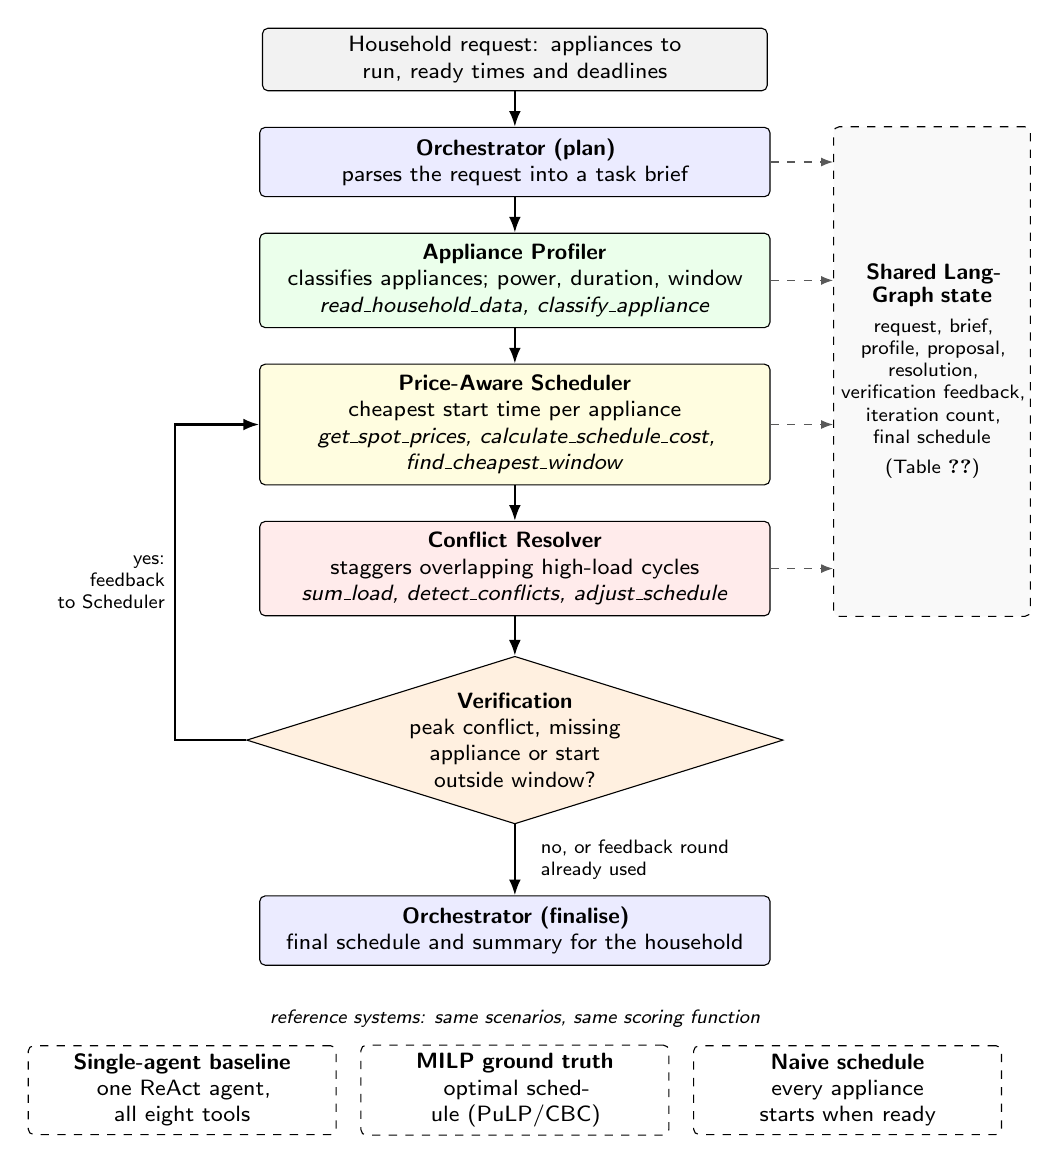
\begin{tikzpicture}[
  font=\sffamily\footnotesize,
  node distance=4.5mm,
  agent/.style={draw, rounded corners=2pt, align=center, text width=6.2cm, inner sep=4pt, fill=#1},
  agent/.default=white,
  io/.style={draw, rounded corners=2pt, align=center, text width=6.2cm, inner sep=3pt, fill=gray!10},
  gate/.style={draw, diamond, aspect=3.2, align=center, inner sep=1pt, fill=orange!12},
  ref/.style={draw, dashed, rounded corners=2pt, align=center, text width=3.7cm, inner sep=3pt},
  flow/.style={-{Latex[length=2mm]}, thick},
  upd/.style={-{Latex[length=1.5mm]}, dashed, gray!70!black},
]
\node[io] (req) {Household request: appliances to run, ready times and deadlines};
\node[agent=blue!8, below=of req] (orch) {\textbf{Orchestrator (plan)}\\
  parses the request into a task brief};
\node[agent=green!8, below=of orch] (prof) {\textbf{Appliance Profiler}\\
  classifies appliances; power, duration, window\\
  \textit{read\_household\_data, classify\_appliance}};
\node[agent=yellow!12, below=of prof] (sched) {\textbf{Price-Aware Scheduler}\\
  cheapest start time per appliance\\
  \textit{get\_spot\_prices, calculate\_schedule\_cost, find\_cheapest\_window}};
\node[agent=red!8, below=of sched] (res) {\textbf{Conflict Resolver}\\
  staggers overlapping high-load cycles\\
  \textit{sum\_load, detect\_conflicts, adjust\_schedule}};
\node[gate, below=5mm of res] (gate) {\textbf{Verification}\\peak conflict, missing\\appliance or start\\outside window?};
\node[agent=blue!8, below=9mm of gate] (fin) {\textbf{Orchestrator (finalise)}\\
  final schedule and summary for the household};
\draw[flow] (req) -- (orch);
\draw[flow] (orch) -- (prof);
\draw[flow] (prof) -- (sched);
\draw[flow] (sched) -- (res);
\draw[flow] (res) -- (gate);
\draw[flow] (gate) -- node[right=2mm, align=left, font=\sffamily\scriptsize] {no, or feedback round\\already used} (fin);
\draw[flow] (gate.west) -- ++(-0.9,0) |- node[pos=0.25, left, align=right, font=\sffamily\scriptsize] {yes:\\feedback\\to Scheduler} (sched.west);
% the shared state spans the four agents; every agent writes to it
\coordinate (stateNW) at ($(orch.north east)+(0.8,0)$);
\coordinate (stateSE) at ($(res.south east)+(3.3,0)$);
\node[draw, dashed, rounded corners=2pt, fill=gray!5, inner sep=0pt, fit=(stateNW)(stateSE)] (state) {};
\node[align=center, text width=2.3cm, font=\sffamily\scriptsize] at (state.center)
      {\textbf{\footnotesize Shared LangGraph state}\\[3pt] request, brief,\\ profile, proposal,\\ resolution,\\
       verification feedback,\\ iteration count,\\ final schedule\\[3pt] (Table~\ref{tab:state})};
\foreach \n in {orch, prof, sched, res} \draw[upd] (\n.east) -- (\n.east -| state.west);
\node[ref, below=10mm of fin] (milp) {\textbf{MILP ground truth}\\optimal schedule (PuLP/CBC)};
\node[ref, left=3mm of milp] (single) {\textbf{Single-agent baseline}\\one ReAct agent, all eight tools};
\node[ref, right=3mm of milp] (naive) {\textbf{Naive schedule}\\every appliance starts when ready};
\node[above=1mm of milp, font=\sffamily\scriptsize\itshape] {reference systems: same scenarios, same scoring function};
\end{tikzpicture}
\caption{Architecture of the hierarchical ReAct multi-agent pipeline.}
\label{fig:arch}
\end{figure}

\begin{table}[h!]
\caption{Fields of the shared LangGraph state.}
\label{tab:state}
\small
\begin{tabularx}{\textwidth}{llX}
\toprule
Field & Written by & Content \\
\midrule
request & caller & the household's scheduling request in natural language \\
brief & Orchestrator & appliance identifiers to schedule and stated constraints \\
profile & Profiler & per appliance: type, flexible or fixed, peak power, cycle duration, earliest start and deadline \\
proposal & Scheduler & start time per appliance, estimated cost and a short justification \\
resolution & Resolver & conflict-free start times, whether conflicts remain, and the changes made \\
verification feedback & verification step & remaining peak conflicts, appliances without a start time and start times outside the user window; empty when the schedule passes \\
iterations & verification step & number of Scheduler--Resolver passes completed (at most two) \\
final, summary & Orchestrator & final start times and the summary shown to the household \\
tool calls, recoveries, errors & all nodes & counters and error messages recorded for the evaluation \\
\bottomrule
\end{tabularx}
\end{table}

\section{Agent specifications}

The \textbf{Orchestrator} receives the household scheduling request,
coordinates the three specialist agents in sequence, and synthesizes the
final output. The Orchestrator does not perform scheduling reasoning
itself, keeping its context window small and decisions reliable across
all scenario types.

The \textbf{Appliance Profiler} reads the household consumption data and
classifies each appliance by shiftability. The classification
distinguishes flexible loads, which have long cycle durations and
user-defined completion windows (washing machines, dishwashers and tumble
dryers), from fixed loads such as refrigerators and microwaves. The Profiler
outputs a structured appliance profile containing power draw in Watts,
typical cycle duration in minutes, and the constraint window for each
flexible load.

The \textbf{Price-Aware Scheduler} receives the appliance profile and
the day-ahead price schedule. It reasons through the price series to
identify the cheapest available window for each flexible appliance
within its constraint envelope and proposes a daily schedule with
per-appliance start times and a total cost estimate.

The \textbf{Conflict Resolver} receives the proposed schedule and checks
for overlapping windows where two or more appliances with high power
draw would run simultaneously, exceeding the household's peak load
threshold. If conflicts exist, the Resolver proposes staggered start
time adjustments that eliminate the conflict while minimizing the
increase in total schedule cost.

Each specialist is a ReAct agent that may only call its own tools and
must end with a structured output (the appliance profile, the proposed
schedule or the resolved schedule), which is validated against a schema
before it is written to the shared state. The agents share a budget of
75 graph steps, divided by workload: 15 for the Profiler, 35 for the
Scheduler and 25 for the Resolver. The Scheduler received the largest
share after the pilot runs showed that it performs most of the tool
calls. When a model replies in prose instead of producing the required
structured output, the agent is resumed from its last state and asked
once more to return the output, at most twice. This rule applies
identically to every agent and model, and every such recovery is
recorded.

Table~\ref{tab:tools} lists the eight tools. They are deterministic
functions over the scenario data, so every number an agent reasons with
comes from a calculation rather than from the language model. No tool
solves the whole problem: \texttt{find\_cheapest\_window} considers one
appliance at a time and ignores both the other appliances and the peak
load limit, so coordinating the appliances is left to the agents.

\begin{table}[h!]
\caption{Tools available to the agents.}
\label{tab:tools}
\small
\begin{tabularx}{\textwidth}{>{\ttfamily\footnotesize\raggedright}p{4.3cm}lX}
\toprule
\normalfont Tool (inputs) & Agent & Output and logic \\
\midrule
read\_household\_data() & Profiler &
  Peak load limit, measured base load range, and for each appliance its
  type, cycle duration, energy, peak power and user window (flexible) or
  rated power (fixed). \\[2pt]
classify\_appliance(\allowbreak appliance\_id) & Profiler &
  Flexible or fixed, with a reason; washing machines, dishwashers and
  tumble dryers are shiftable cycle loads. \\[2pt]
get\_spot\_prices(\allowbreak from\_time, to\_time) & Scheduler &
  Consumer price in c/kWh for every 15-minute slot, optionally for a time
  range. \\[2pt]
calculate\_\allowbreak schedule\_cost(\allowbreak appliance\_id, start\_time) & Scheduler &
  Cost of one cycle started at the given time (power profile $\times$
  price $\times$ 0.25\,h, summed over the cycle), its end time, and
  whether it lies within the user window. \\[2pt]
find\_cheapest\_\allowbreak window(\allowbreak appliance\_id, top\_k) & Scheduler &
  The $k$ cheapest start times within the user window for one appliance,
  found by evaluating every valid start. \\[2pt]
sum\_load(schedule) & Resolver &
  Maximum total household load (base load plus scheduled cycles) and the
  five highest slots, compared with the limit. \\[2pt]
detect\_conflicts(\allowbreak schedule) & Resolver &
  Time ranges in which the total load exceeds the limit and the
  appliances running then, or confirmation that there is no conflict. \\[2pt]
adjust\_schedule(\allowbreak schedule, appliance\_id, new\_start\_time) & Resolver &
  Moves one appliance and reports the cost change, the window check and
  any remaining overload. Without a start time, it moves the appliance to
  its cheapest start at which it causes no overload, keeping the others
  fixed, and lists alternatives. \\
\bottomrule
\end{tabularx}
\end{table}

\section{Single-agent baseline}

The single-agent baseline is one ReAct agent, built with LangChain's
\texttt{create\_agent} on the LangGraph runtime, with access to all eight
tools of Table~\ref{tab:tools}. It receives the same household request as
the pipeline, and its system prompt is assembled from the same role
instructions that the three specialists receive, so both designs have
the same domain knowledge. Its step budget of 75 equals the combined
budget of the specialists, and the same structured output schema and
recovery rule apply. The only controlled difference between the baseline
and the artifact is therefore the presence or absence of role
specialization.

The baseline and the pipeline were validated on six pilot scenarios, one
per scenario type, before the full evaluation (Section~\ref{sec:demonstration}).

\section{MILP ground truth solver}

The MILP solver computes the mathematically optimal schedule for each
scenario. The day is divided into slots $t \in \mathcal{T} =
\{0, \dots, 95\}$ of $\Delta = 0.25$\,h. Each flexible appliance
$a \in \mathcal{A}$ has a power profile $p_{a,0}, \dots, p_{a,d_a-1}$ in
kW over its cycle of $d_a$ slots, an earliest start slot $e_a$ and a
deadline slot $\ell_a$ by which the cycle must end. Its admissible start
slots are
\[
\mathcal{S}_a = \{\, s \in \mathbb{Z} : e_a \le s \le \ell_a - d_a \,\}.
\]
The model uses binary start variables $x_{a,s} \in \{0,1\}$, equal to one
if appliance $a$ starts in slot $s \in \mathcal{S}_a$. With the consumer
price $\pi_t$ in \euro/kWh, the base load $b_t$ in kW and the household
peak limit $\bar{P}$ in kW, the model is
\begin{align}
\min_{x} \quad & \sum_{a \in \mathcal{A}} \sum_{s \in \mathcal{S}_a}
  c_{a,s}\, x_{a,s},
  \qquad c_{a,s} = \Delta \sum_{k=0}^{d_a-1} p_{a,k}\, \pi_{s+k},
  \label{eq:milp-objective} \\
\text{s.t.} \quad & \sum_{s \in \mathcal{S}_a} x_{a,s} = 1
  \qquad \forall a \in \mathcal{A},
  \label{eq:milp-one-start} \\
& b_t + \sum_{a \in \mathcal{A}} \; \sum_{\substack{s \in \mathcal{S}_a \\ 0 \le t-s < d_a}}
  p_{a,t-s}\, x_{a,s} \le \bar{P}
  \qquad \forall t \in \mathcal{T},
  \label{eq:milp-peak} \\
& x_{a,s} \in \{0,1\}
  \qquad \forall a \in \mathcal{A},\ s \in \mathcal{S}_a .
  \nonumber
\end{align}
The objective~\eqref{eq:milp-objective} is the consumer cost of the
flexible cycles, with $c_{a,s}$ the precomputed cost of starting
appliance $a$ in slot $s$. Constraint~\eqref{eq:milp-one-start} requires
exactly one cycle per appliance, and constraint~\eqref{eq:milp-peak}
keeps the total household load within the peak limit in every slot.
Because a decision fixes the start of a whole cycle, each cycle runs
without interruption once started, and restricting the variables to
$\mathcal{S}_a$ keeps every cycle within its user window, so neither
property needs a separate constraint. The model is solved with PuLP and
the CBC solver in well under a second per scenario. Its correctness was
verified against exhaustive enumeration of all start combinations on
small scenarios, and it is also used during benchmark construction to
confirm that every scenario has a feasible schedule.

\section{Technology stack}

Table~\ref{tab:stack} lists the software used to build and evaluate the
artifact, with the versions used for the reported results. All components
except the commercial language model are open source. The API cost of
the commercial model is an outcome of the evaluation and is reported with
the results in Chapter~5.

\begin{table}[h!]
\caption{Technology stack.}
\label{tab:stack}
\small
\begin{tabularx}{\textwidth}{l>{\raggedright\arraybackslash}p{4.0cm}X}
\toprule
Component & Tool and version & Purpose \\
\midrule
Programming language & Python 3.12 & implementation of the artifact, baselines and analysis \\[2pt]
Agent orchestration & LangGraph 1.2, LangChain 1.4 & state graph of the pipeline, ReAct agents, tool calling and schema-validated outputs \\[2pt]
Commercial LLM & GPT-4o-mini (snapshot 2024-07-18), OpenAI API & cloud model for both designs \\[2pt]
Open-weight LLM & gpt-oss-20b, Ollama 0.34 & open-weight model hosted on local hardware (SQ3) \\[2pt]
MILP solver & PuLP 3.3 with CBC & optimal reference schedules \\[2pt]
Data processing & pandas 3.0, NumPy 2.5 & REFIT cycle extraction, price series and scenario construction \\[2pt]
Tracing & LangSmith & recording the reasoning trace and tool calls of every run \\[2pt]
Statistics & SciPy 1.18 & Wilcoxon signed-rank test, effect size and Spearman correlation \\
\bottomrule
\end{tabularx}
\end{table}

% ════════════════════════════════════════════════════════════════════════════
\chapter{Evaluation and Results}

This chapter presents the evaluation of the artifact, corresponding to
DSR Phases 4 and 5. Section~\ref{sec:dataset} describes the benchmark:
the appliance and price data and the construction of the 48 evaluation
scenarios across six price-volatility types. Section~\ref{sec:resolution}
uses the MILP solver alone to examine Finland's move to fifteen-minute
electricity prices, quantifying how much of the achievable scheduling
saving depends on fifteen-minute rather than hourly price information;
this establishes where differences between schedulers can be expected
before any agent is evaluated. Section~\ref{sec:demonstration} reports
the demonstration of the pipeline on representative scenarios (DSR
Phase 4). Sections~\ref{sec:quantitative} and~\ref{sec:statistics}
compare the optimality gaps of the multi-agent pipeline and the
single-agent baseline across all scenarios and test the difference with
the Wilcoxon signed-rank test. Section~\ref{sec:baselines} compares
both designs with two simpler baselines, a rule-based smart timer and a
language model without tools. Section~\ref{sec:confirmatory} repeats
the tests of H1 and H2 on the held-out fifteen-minute benchmark, as fixed
in the pre-registration. Section~\ref{sec:per-appliance} breaks
the cost savings down by appliance type. The agent results in
Sections~\ref{sec:demonstration}--\ref{sec:per-appliance} are pending
the full evaluation runs.

\section{Dataset and scenario design}
\label{sec:dataset}

The evaluation benchmark combines real appliance consumption profiles
from UK households with real Finnish day-ahead electricity prices. Each
of the 48 scenarios describes one day in 96 fifteen-minute slots
(00:00--24:00 local time) and consists of a price curve, a household
base load, a set of flexible appliance cycles with user time windows, and
a household peak load limit. The benchmark is generated by a
deterministic, seeded build procedure, so it can be reproduced exactly
from the source data.

\subsection{Appliance data}

Appliance profiles are drawn from the cleaned REFIT Electrical Load
Measurements dataset (Murray et al., 2017; Murray \& Stankovic, 2016),
which records the whole-house aggregate and nine individually monitored
appliances at 8-second intervals in 20 UK households between 2013 and
2015. The cleaned release corrects timestamps for daylight saving time
and re-aligns appliance monitor columns where a monitor was moved between
appliances during the study. The appliance-to-column mapping follows
the dataset documentation.

Eighteen households are used. House 12 is excluded because it has no
monitored washing machine, dishwasher or tumble dryer. House 19 is
excluded after inspection: its washing-machine monitor recorded no
heating phase in any of its 246 detected cycles (no fifteen-minute mean
above 1.2\,kW, against 22--70\,\% of cycles in the other households),
so its profiles do not represent the water-heating load that dominates
the cost and peak demand of a wash. Washer-dryers (houses 1, 8, 9 and
18) are not used as profiles, because they run washing and drying as a
single cycle; their consumption is nevertheless removed from the base
load.

Individual appliance cycles are extracted from each monitor by
thresholding the one-minute mean power at 20\,W and merging pauses
shorter than 30 minutes for dishwashers (whose programmes contain a
passive drying pause) and 15 minutes for washing machines and tumble
dryers (which are often reloaded within minutes). Cycles shorter than
20 minutes, longer than 300 minutes or below 0.1\,kWh are discarded, and
each remaining cycle is converted into a fifteen-minute mean power
profile. This yields 6,172 washing-machine cycles from 19 monitored
machines, 4,702 dishwasher cycles from 15 machines and 1,940
tumble-dryer cycles from 7 machines. To prevent heavily used appliances
from dominating the benchmark, a scenario first draws a monitored
appliance of the required type and then one of its cycles. The household
base load is the median, per fifteen-minute slot of the day, of the
aggregate minus all shiftable appliance monitors, computed after
discarding readings that the dataset flags as inconsistent (sub-metered
sum exceeding the aggregate).

\subsection{Electricity price data}

Day-ahead spot prices for the Nord Pool FI bidding zone were obtained
for 1 January 2022 to 24 September 2026 from the public Sähkötin price
service, which republishes Nord Pool data (Pakastin Oy, 2026). The
values are in EUR/MWh excluding VAT and were verified against an
independent source for the December 2022 crisis period. The service
provides hourly values, which are repeated across the four fifteen-minute
slots of each hour; days with a daylight-saving transition are dropped,
leaving 1,718 complete days.

Scheduling cost is computed with the consumer price rather than the raw
spot price. For spot price $s$, the consumer price per kWh is
\[
p = (s + m + d + \tau)(1 + v),
\]
with a retail margin $m = 0.5$\,c/kWh, a distribution fee $d =
5.0$\,c/kWh, the electricity tax $\tau = 2.253$\,c/kWh and VAT $v =
25.5\,\%$. These are representative values for a Finnish household on a
spot-price contract; a single VAT rate is applied to all days so that
scenarios from different periods remain comparable. Using the consumer
price keeps costs positive on days with negative spot prices, which
keeps the optimality gap defined in Section~\ref{sec:evaluation} meaningful. Only the
energy of the flexible appliances is costed, since the base load costs
the same under every schedule.

\subsection{Scenario construction}

Table~\ref{tab:scenarios} summarises the six scenario types. Days are
assigned to types by the within-day standard deviation of the spot
price. Types A and B use disjoint days from the lowest quartile among
days without negative prices, type C uses days between the 40th and
60th percentiles, and type D uses days in the top 15\,\% that fall in
December--February. Type E uses days from December 2022, sampled from the
16 days with the highest maximum price. Type F uses days with at least
two hours of negative prices. Eight days are sampled per type.

Types C--F need up to five loads, while REFIT provides three flexible
appliance types; a scenario may therefore contain two cycles of the same
type, such as two washing loads. Each appliance has a user window
(earliest start and deadline), and its naive start time is the earliest
start. Types A--C use windows opening between 06:00 and 12:00 and lasting
8--14 hours. In type D all five appliances share one window from
08:00--10:00 until 22:00--24:00, so their cheapest start times coincide.
In type E each appliance becomes ready 0--2 hours before the day's
highest daytime price and has 4--8 hours of slack beyond its cycle, so
the naive schedule runs into the price spike while avoiding it remains
possible. This reflects that price spikes coincide with evening demand
peaks, when households tend to start appliances. Type F windows open
between 00:00 and 04:00 and last until midnight.

The household peak load limit, including the base load, is 3.5\,kW. It
represents a household power cap, for example one induced by a
power-based distribution tariff, rather than the main fuse (typically
3\,$\times$\,25\,A, about 17\,kW), which would never bind for these
appliances. The build procedure verifies with the MILP solver that every
scenario has a feasible schedule; this held for all 48 scenarios
without relaxing the limit. Table~\ref{tab:benchmark} reports the
resulting characteristics per type. A scenario requires coordination
when running every appliance at its individually cheapest start time
exceeds the peak limit; these 28 scenarios form the basis of the
conflict resolution rate.

\begin{table}[h!]
\caption{Evaluation scenario design.}
\label{tab:scenarios}
\small
\begin{tabularx}{\textwidth}{llXcX}
\toprule
Type & Price regime & Appliances & Inst. & Research purpose \\
\midrule
A & Stable, low volatility &
  2 appliances: dishwasher + washing machine & 8 &
  Baseline check: both systems should perform well \\[3pt]
B & Stable, low volatility &
  3 appliances: dishwasher + washing machine + tumble dryer & 8 &
  Tests three-way conflict resolution \\[3pt]
C & Moderate volatility &
  3 to 5 appliances mixed & 8 &
  Tests price-signal responsiveness \\[3pt]
D & High volatility, winter peak &
  5 appliances, overlapping constraints & 8 &
  Most financially consequential condition \\[3pt]
E & Price spike (Dec 2022 crisis) &
  3 appliances, ready 0--2\,h before the daily price peak, 4--8\,h slack & 8 &
  Extreme Finnish price event robustness \\[3pt]
F & Negative spot price (surplus) &
  4 appliances, flexible windows & 8 &
  Tests exploitation of zero-cost windows \\
\bottomrule
\end{tabularx}
\end{table}

\begin{table}[h!]
\caption{Benchmark characteristics per scenario type.}
\label{tab:benchmark}
\small
\begin{tabularx}{\textwidth}{l>{\raggedright\arraybackslash}Xcccc}
\toprule
Type & Price days & \makecell{Mean\\appliances} & \makecell{Require\\coordination} &
  \makecell{Naive schedule\\within limit} & \makecell{MILP saving\\vs.\ naive} \\
\midrule
A & 2022--2026 & 2.0 & 1/8 & 8/8 & 10.2\,\% \\
B & 2023--2026 & 3.0 & 4/8 & 7/8 & 4.3\,\% \\
C & 2023--2026 & 3.4 & 5/8 & 6/8 & 19.9\,\% \\
D & 2022--2026 (Dec--Feb) & 5.0 & 8/8 & 0/8 & 37.0\,\% \\
E & 1--14 Dec 2022 & 3.0 & 4/8 & 3/8 & 14.4\,\% \\
F & 2023--2025 & 4.0 & 6/8 & 5/8 & 7.8\,\% \\
\midrule
All & & 3.4 & 28/48 & 29/48 & \\
\bottomrule
\end{tabularx}
\end{table}

\section{Value of 15-minute price information}
\label{sec:resolution}

Since 1 October 2025 the Nord Pool day-ahead market settles Finnish
electricity in fifteen-minute periods. The main benchmark uses hourly
prices, because its type E days date from the 2022 energy crisis. To
examine the new market design, a second set of 48 scenarios (Q-A01 to
Q-F08) was built with the same procedure from native fifteen-minute FI
prices for 1 October 2025 to 25 September 2026 (358 complete days),
obtained from the public price service of the Estonian transmission
system operator, which republishes Nord Pool data (Elering AS, 2026).
Its hourly averages match the hourly series used in
Section~\ref{sec:dataset}. Because this period contains no crisis month,
its type E days are drawn from the 16 days with the highest peak price
(up to 65\,c/kWh), and no day is used by more than one type. Prices
genuinely vary within the hour: in 98\,\% of hours the four quarter-hour
prices differ, with a median spread of 0.75\,c/kWh.

For each Q scenario, two optimal schedules were computed with the MILP
solver. The first is planned on the real fifteen-minute prices. The
second is planned on hourly averages, which is all the price information
a household had before the switch, and is then settled at the real
fifteen-minute prices. Hourly prices make the four quarters of an hour
tie, so ties are broken towards the earliest start. The cost difference
between the two schedules is the saving that is only reachable with
fifteen-minute price information. Table~\ref{tab:resolution} reports the
savings of both schedules relative to the naive schedule, the
additional cost reduction from fifteen-minute information, and the share
of the achievable saving that requires it; the ``All'' row weights
scenarios by their cost.

% Generated by `hems resolution` -- do not edit by hand.
\begin{table}[h!]
\caption{Optimal schedule cost with hourly vs.\ 15-minute price information (MILP, Q scenarios).}
\label{tab:resolution}
\small
\begin{tabular*}{\textwidth}{@{\extracolsep{\fill}}lcccccc}
\toprule
Type & \makecell{Intra-hour\\spread\\(c/kWh)} & \makecell{Saving,\\hourly\\plan} & \makecell{Saving,\\15-min\\plan} & \makecell{Additional\\cost\\reduction} & \makecell{Share of\\saving\\needing\\15-min} & \makecell{Scenarios\\improved} \\
\midrule
A & 0.41 & 4.1\,\% & 4.2\,\% & 0.1\,\% & 2.4\,\% & 5/8 \\
B & 0.33 & 3.2\,\% & 3.4\,\% & 0.3\,\% & 6.4\,\% & 8/8 \\
C & 1.37 & 7.1\,\% & 8.6\,\% & 1.7\,\% & 16.4\,\% & 8/8 \\
D & 4.96 & 27.6\,\% & 28.6\,\% & 1.4\,\% & 3.5\,\% & 8/8 \\
E & 4.91 & 35.4\,\% & 37.0\,\% & 2.1\,\% & 2.8\,\% & 6/8 \\
F & 0.21 & 4.6\,\% & 4.7\,\% & 0.1\,\% & 1.7\,\% & 4/8 \\
\midrule
All & 2.03 & 23.7\,\% & 24.7\,\% & 1.2\,\% & 3.7\,\% & 39/48 \\
\bottomrule
\end{tabular*}
\end{table}


Fifteen-minute price information lowers the optimal cost in 39 of the 48
scenarios, but the effect is modest: 1.2\,\% overall, or 3.7\,\% of the
achievable saving. The remaining 96\,\% of the saving is available to a
scheduler that plans on hourly prices, since most of the value lies in
moving appliance cycles between hours rather than between quarters of an
hour. The additional reduction grows with the intra-hour price spread
(Spearman $\rho = 0.66$ across scenarios) and is largest on volatile
days: 1.4\,\% in type D, 2.1\,\% in type E, and 10.2\,\% in the single
largest case (Q-E03, 17 October 2025). Type C shows the largest relative
share (16.4\,\%), because its hourly price differences are small, so
intra-hour variation forms a larger part of the opportunity. In absolute
terms the gain is about one cent per household per day for the two to
five cycles scheduled, and about three cents on type D days. The
schedules nevertheless differ: 110 of the 163 appliance start times
change between the two plans. These results indicate that the hourly
main benchmark captures most of the scheduling problem, while any
difference between the agents under fifteen-minute prices is expected
to appear mainly in types C, D and E.

\section{Demonstration results}
\label{sec:demonstration}
Work in progress.

\section{Quantitative results}
\label{sec:quantitative}
Work in progress.

\section{Statistical analysis}
\label{sec:statistics}

% Hand-typed from `hems analyze` (results/tables/equivalence.csv, efficiency_tests.csv),
% GPT-4o-mini only. Update when the gpt-oss-20b runs are complete.
This section reports the tests described in Section~\ref{sec:evaluation}
for GPT-4o-mini on the main benchmark, with the mean over three runs per
scenario as the paired observation ($N = 48$). These results are
exploratory; the pre-registered confirmatory results are reported in
Section~\ref{sec:confirmatory}. The results for gpt-oss-20b are added
when its runs are complete.

\paragraph{Schedule quality.} The multi-agent pipeline reached a mean
optimality gap of 1.25\,\% and the single agent 1.43\,\%. The Wilcoxon
signed-rank test finds no significant difference ($W = 449$,
$Z = -0.14$, $p = 0.89$, $r = 0.02$), and the median paired difference
is zero, because both designs reach the same cost in most scenarios. The
equivalence test shows that this is not merely a lack of evidence. The
mean paired difference is $-0.18$ percentage points, with a 90\,\%
confidence interval of $[-0.71, 0.35]$, which lies inside the primary
margin of $\pm 1$ percentage point (Table~\ref{tab:equivalence}). The two
designs are therefore equivalent in schedule quality within one
percentage point of the optimum. At the narrower margin of 0.5
percentage points the $t$ version of the test does not conclude
equivalence, because a few scenarios with large differences in either
direction widen the interval, although the Wilcoxon version does.

\begin{table}[h!]
\caption{Equivalence test (TOST) of the optimality gap, multi-agent vs.\ single-agent (GPT-4o-mini, $N = 48$).}
\label{tab:equivalence}
\small
\begin{tabular*}{\textwidth}{@{\extracolsep{\fill}}lccc}
\toprule
Margin & $p$, paired $t$ TOST & $p$, Wilcoxon TOST & Equivalent \\
\midrule
$\pm 0.5$ percentage points & 0.156 & $<$\,0.001 & No \\
$\pm 1$ percentage point (primary) & 0.006 & $<$\,0.001 & Yes \\
$\pm 2$ percentage points & $<$\,0.001 & $<$\,0.001 & Yes \\
\bottomrule
\end{tabular*}
\end{table}

\paragraph{Efficiency.} The two designs differ significantly in every
efficiency measure (Table~\ref{tab:efficiency-tests}). The pipeline used
34\,\% fewer input tokens, because each specialist works with a short
context and only its own tools, while the single agent carries the
entire conversation and all eight tool descriptions through every step.
It produced 83\,\% more output tokens and made 23\,\% more tool calls,
since four agents each write their own structured output and call their
tools separately. Input tokens dominate the price, so the API cost per run was
21\,\% lower for the pipeline, and lower in 35 of the 48 scenarios. The
sequential hand-offs made the pipeline 69\,\% slower, with a mean of
21.4 seconds against 12.7 seconds, and it was faster in only two
scenarios.

\begin{table}[h!]
\caption{Efficiency per run, multi-agent vs.\ single-agent (GPT-4o-mini, means over $N = 48$ scenarios, Wilcoxon signed-rank test).}
\label{tab:efficiency-tests}
\small
\begin{tabular*}{\textwidth}{@{\extracolsep{\fill}}lcccccc}
\toprule
Measure & \makecell{Single\\agent} & \makecell{Multi-\\agent} & Difference & \makecell{Multi-agent\\lower} & $p$ & $r$ \\
\midrule
Input tokens & 21\,686 & 14\,292 & $-34$\,\% & 43/48 & $<$\,0.001 & 0.79 \\
Output tokens & 661 & 1\,208 & $+83$\,\% & 1/48 & $<$\,0.001 & 0.87 \\
Total tokens & 22\,347 & 15\,500 & $-31$\,\% & 40/48 & $<$\,0.001 & 0.75 \\
API cost (USD) & 0.0037 & 0.0029 & $-21$\,\% & 35/48 & $<$\,0.001 & 0.54 \\
Latency (s) & 12.7 & 21.4 & $+69$\,\% & 2/48 & $<$\,0.001 & 0.86 \\
Tool calls & 16.5 & 20.3 & $+23$\,\% & 1/48 & $<$\,0.001 & 0.81 \\
\bottomrule
\end{tabular*}
\end{table}

Taken together, decomposing the task into specialist agents did not
lower the cost of the schedules, but it reached the same quality with
about a third fewer tokens and a fifth lower inference cost, at the price
of a longer response time.

\section{Comparison with simpler baselines}
\label{sec:baselines}

% Hand-typed from `hems analyze --runs results/runs.jsonl results/baselines.jsonl` (GPT-4o-mini).
Table~\ref{tab:baselines} compares the two agent designs with the smart
timer and the no-tools baseline. All systems that use a language model
use GPT-4o-mini.

\begin{table}[h!]
\caption{Agent designs and simpler baselines (GPT-4o-mini, 48 scenarios).}
\label{tab:baselines}
\small
\begin{tabular*}{\textwidth}{@{\extracolsep{\fill}}lcccccc}
\toprule
System & \makecell{Feasible\\runs} & \makecell{Mean\\gap} & \makecell{Median\\gap} & \makecell{Gap,\\type D} & \makecell{Savings\\captured} & \makecell{Time\\per run} \\
\midrule
Smart timer (no language model) & 48/48 & 0.23\,\% & 0.00\,\% & 1.2\,\% & 99\,\% & $<$\,0.01\,s \\
Multi-agent pipeline & 144/144 & 1.25\,\% & 0.01\,\% & 5.9\,\% & 94\,\% & 21.4\,s \\
Single agent & 143/144 & 1.43\,\% & 0.00\,\% & 6.5\,\% & 93\,\% & 12.7\,s \\
No-tools language model & 126/144 & 23.1\,\% & 11.9\,\% & 66.0\,\% & $-17$\,\% & 2.0\,s \\
\bottomrule
\end{tabular*}
\end{table}

Without tools, GPT-4o-mini schedules poorly. Its mean optimality gap is
23.1\,\%, and 18 of its 144 schedules are infeasible: 14 exceed the peak
limit and 4 start a cycle outside its window. A further 22 of its
feasible schedules cost more than starting every appliance as soon as it
is ready, so on average it captures less than none of the achievable
saving. Both agent designs are significantly better (Wilcoxon
$p < 0.001$, $r = 0.87$ for each), with median paired differences of
10.8 percentage points for the single agent and 11.4 for the pipeline.
The same model that fails to schedule from a single prompt comes close to
the optimum when it can query prices, costs and loads through tools and
check its own work. Tool use, rather than the language model's own
calculation, is therefore what makes the agents viable.

The smart timer, however, outperforms both agent designs. It finds a
feasible schedule in every scenario, is optimal in 30 of the 48, and its
largest gap is 3.7\,\% (D04). Both agent designs have significantly
larger gaps than the timer (single agent $p < 0.001$, $r = 0.63$;
pipeline $p < 0.001$, $r = 0.68$). The difference is concentrated in
type D, where the timer's mean gap is 1.2\,\% against 5.9\,\% for the
pipeline and 6.5\,\% for the single agent. The median paired differences
are small (0.002 percentage points for the single agent and 0.017 for the
pipeline), because in most scenarios all three systems reach the optimum
or come very close to it. The timer needs no language model, runs in
about two milliseconds and has no inference cost. In this benchmark,
where the power profile and window of every appliance are known exactly
and the horizon is one day, placing the appliances one at a time is
almost always enough. The agents come within about one percentage point
of this rule but do not improve on it. What they add is the ability to
start from a request written in natural language rather than from
structured appliance data, and to explain the schedule they produce. The
Discussion returns to what this implies for the artifact.

\section{Confirmatory evaluation}
\label{sec:confirmatory}
Work in progress. This section will report the pre-registered tests of
H1 and H2 on the held-out fifteen-minute benchmark.

\section{Per-appliance breakdown}
\label{sec:per-appliance}
Work in progress.

% ════════════════════════════════════════════════════════════════════════════
\chapter{Discussion}

Work in progress. This chapter will interpret the results in relation to
the research questions, connect findings to the agentic AI trends
reviewed in Chapter~2, and address the limitations and directions for
future research.

\section{Interpretation of research questions}
Work in progress.

\section{Agents compared with simpler schedulers}

The comparison with simpler baselines in Section~\ref{sec:baselines}
places the results in context, and two findings stand out. First, tool
use is essential. The same language model that captures more than
90\,\% of the achievable saving as an agent does worse than no
scheduling at all when it has to work out the schedule in a single
answer. This agrees with the motivation for ReAct (Yao et al., 2023),
in which reasoning is grounded in the observations returned by actions
instead of being carried out unaided. It indicates that the role of the
language model in the pipeline is to decide which calculations to
request and how to combine their results, not to perform the
calculations itself.

Second, on well-specified single-day problems a rule-based smart timer
is slightly better than either agent design and costs almost nothing to
run. For a household whose appliances and time windows are already known
to a home energy management system in structured form, the evidence
therefore does not support replacing such a rule with a language model
agent on cost grounds. The case for the agents rests on the interface
instead. They accept a request written in everyday language, check it
against the household data and explain the resulting schedule, while
keeping its cost within about one percentage point of the rule. The
benchmark does not test this advantage directly, because its requests
are regular enough to be turned into the timer's input without
difficulty. Requests that are informal, incomplete or contradictory, and
a measure of how accurately each system turns them into constraints,
would be the most direct way to establish where the agents add value.

\section{Limitations}

Several limitations of this study warrant acknowledgement. First, the
evaluation is entirely simulation-based using historical data. While the
use of real consumption profiles and real Nord Pool FI prices provides
stronger ecological validity than synthetic scenarios, the study does
not evaluate the pipeline in a live deployment where appliance states
change dynamically and user preferences may deviate from scripted
constraint windows. Second, the REFIT dataset was collected from UK
homes between 2013 and 2015 and may not fully reflect the appliance
configurations and usage patterns of contemporary Finnish households.
Third, LLM outputs are non-deterministic: two runs of the same scenario
may produce different schedules. To mitigate this, each scenario is run
three times and results are averaged, but residual variance from
non-determinism remains. Fourth, the study evaluates only three
appliance types; generalizing findings to electric vehicle chargers,
heat pumps, or battery storage requires additional evaluation. Fifth,
the benchmark requests are generated from a template and state the
window of every appliance explicitly. They therefore do not test the
agents' ability to interpret informal requests, which is where their
advantage over rule-based scheduling is expected, and on these
well-specified problems a rule-based smart timer outperforms both agent
designs (Section~\ref{sec:baselines}).

\section{Future research}

Several directions for future research emerge from this study. First,
extending the pipeline to thermal loads such as electric space heating,
heat pumps and domestic hot water systems would address the gap
explicitly identified by El Makroum et al. (2026). Second,
implementing the price API and data reader as MCP servers would enable
reuse by future researchers without custom integration code,
contributing to the emerging standardization of agent tool interfaces.
Third, a live deployment study involving Finnish households on
spot-price contracts would provide ecological validity that
simulation-based evaluation cannot. Fourth, extending the multi-LLM
comparison to include Qwen-3-32B and Phi-4 would provide a more
complete picture of the SLM landscape for residential scheduling tasks.
Fifth, a benchmark of informal household requests with annotated
constraints would test the agents where a rule-based scheduler cannot
operate, by measuring how accurately each system turns such requests
into a correct schedule.

% ════════════════════════════════════════════════════════════════════════════
\chapter{Conclusions}

Work in progress. This chapter will summarize the main contributions of
the thesis, explicitly answer the RQ and SQ1 to SQ4 using evidence from
Chapter~5, and state the implications for academic research on
multi-agent LLM systems and practical deployment of intelligent demand
flexibility tools in Finnish residential settings.

% ════════════════════════════════════════════════════════════════════════════
\chapter*{References}
\addcontentsline{toc}{chapter}{References}

\begin{hangparas}{0.7cm}{1}

Anthropic. (2024). \textit{Model Context Protocol}.
\url{https://modelcontextprotocol.io}

Anthropic. (2026). \textit{AI agents in 2026: Key trends and
organizational adoption patterns}. Anthropic Research Report.

Beaudin, M., \& Zareipour, H. (2015). Home energy management systems: A
review of modelling and complexity. \textit{Renewable and Sustainable
Energy Reviews, 45}, 318--335.

Elering AS. (2026). \textit{Nord Pool day-ahead prices, bidding zone FI}
[Data service; data owner Nord Pool]. Retrieved 26 September 2026, from
\url{https://dashboard.elering.ee/api/nps/price}

El Makroum, M., et al. (2026). Agentic AI home energy management system:
A large language model framework for residential load scheduling.
\textit{ScienceDirect}. arXiv:2510.26603.

Haakana, J., Lassila, J., Kaipia, T., \& Partanen, J. (2025). Effects
of extreme spot market prices on the electrical power system: Lessons
from the Finnish distribution system. \textit{IET Generation,
Transmission and Distribution}.

Han, S., Zhang, Q., Zhao, L., Xu, R., Peng, W., \& Yang, H. (2024). LLM
multi-agent systems: Challenges and open problems. arXiv:2402.03578.

Hevner, A. R., March, S. T., Park, J., \& Ram, S. (2004). Design
science in information systems research. \textit{MIS Quarterly, 28}(1),
75--105.

Hong, S., Zhuge, M., Chen, J., Zheng, X., Cheng, Y., Zhang, C., \&
Schmidhuber, J. (2023). MetaGPT: Meta programming for a multi-agent
collaborative framework. arXiv:2308.00352.

Jonah, N., et al. (2026). LLMs for agentic home energy management.
arXiv:2607.04569.

Lakens, D. (2017). Equivalence tests: A practical primer for \textit{t}
tests, correlations, and meta-analyses. \textit{Social Psychological and
Personality Science, 8}(4), 355--362.
\url{https://doi.org/10.1177/1948550617697177}

March, S. T., \& Smith, G. F. (1995). Design and natural science
research on information technology. \textit{Decision Support Systems,
15}(4), 251--266.

Mocanu, E., Mocanu, D. C., Nguyen, P. H., Liotta, A., Webber, M. E.,
Gibescu, M., \& Slootweg, J. G. (2018). On-line building energy
optimization using deep reinforcement learning. \textit{IEEE
Transactions on Smart Grid, 10}(4), 3698--3708.

Moradzadeh, B., \& Tomsovic, K. (2013). Two-stage residential energy
management considering network operational constraints. \textit{IEEE
Transactions on Smart Grid, 4}(4), 2339--2346.

Murray, D., \& Stankovic, L. (2016). \textit{REFIT: Electrical load
measurements (cleaned)} [Data set]. University of Strathclyde.
\url{https://doi.org/10.15129/9ab14b0e-19ac-4279-938f-27f643078cec}

Murray, D., Stankovic, L., \& Stankovic, V. (2017). An electrical load
measurements dataset of United Kingdom households from a two-year
longitudinal study. \textit{Scientific Data, 4}, 160122.
\url{https://doi.org/10.1038/sdata.2016.122}

NVIDIA Corporation. (2025). \textit{Efficient inference with small
language models}. NVIDIA Technical Position Paper.

Numminen, S., et al. (2026). \textit{Energy poverty is not recognized in
Finland}. Aalto University Research Report.

Pakastin Oy. (2026). \textit{Sähkötin: Nord Pool FI day-ahead spot
prices} [Data service]. Retrieved 25 September 2026, from
\url{https://sahkotin.fi}

Peffers, K., Tuunanen, T., Rothenberger, M. A., \& Chatterjee, S.
(2007). A design science research methodology for information systems
research. \textit{Journal of Management Information Systems, 24}(3),
45--77.

Schuirmann, D. J. (1987). A comparison of the two one-sided tests
procedure and the power approach for assessing the equivalence of
average bioavailability. \textit{Journal of Pharmacokinetics and
Biopharmaceutics, 15}(6), 657--680.
\url{https://doi.org/10.1007/BF01068419}

Yao, S., Zhao, J., Yu, D., Du, N., Shafran, I., Narasimhan, K., \& Cao,
Y. (2023). ReAct: Synergizing reasoning and acting in language models.
\textit{International Conference on Learning Representations (ICLR
2023)}. arXiv:2210.03629.

\end{hangparas}

\end{document}
